\documentclass[11pt,a4paper]{article}
\usepackage[margin=2.5cm]{geometry}
\usepackage{setspace}\onehalfspacing
\usepackage{amsmath,amssymb}
\usepackage{graphicx}
\usepackage{booktabs}
\usepackage{array}
\usepackage{caption}
\usepackage{subcaption}
\usepackage{hyperref}
\usepackage{xcolor}
\usepackage{tikz}
\usetikzlibrary{positioning,shapes.geometric,arrows.meta,fit,calc}
\usepackage{pgfplots}\pgfplotsset{compat=1.18}

\hypersetup{colorlinks=true,linkcolor=black,citecolor=black,urlcolor=blue}

\title{\textbf{Assignment 5: Deep Learning for Seed Counting and Neural Style Transfer}\\[0.5em]
\large AgriVision Technologies --- Final Phase Report}
\author{Student Report}
\date{May 2026}

\begin{document}
\maketitle
\tableofcontents
\newpage

%%=============================================================
\section{Executive Summary}
%%=============================================================

This report presents two deep learning systems developed for AgriVision Technologies.
The first is a convolutional neural network (CNN) trained from scratch on the seed-counting
dataset introduced in Assignment 2, replacing the prior clustering and edge-detection
approaches. The second is a video stylisation pipeline combining a trained human-matting
model with Neural Style Transfer (NST) applied to a self-recorded video.

For the seed task, the best three-block CNN (Model A) achieves a validation MAE of 2.44
seeds per image in the ablation study, compared to errors exceeding 15 seeds per image in
high-density conditions with the Assignment 2 method. The single most consequential
finding is that SGD with momentum outperforms Adam by a factor of 5.5 in MAE on this
dataset; architectural choices (depth, residual connections, activation function) provide
further but smaller gains. The four-block model (Model B) does not improve upon Model A,
indicating that the primary bottleneck is data quantity rather than model capacity.

For Task 2, the matting model targets IoU $\geq 0.85$ on the AISegment validation split
(\textbf{[INSERT after training]}), and the NST pipeline produces three stylised video
variants. In terms of deployment cost, the CNN seed counter runs in under 5\,ms per image
on a GPU, making it viable for real-time field use. The matting and NST pipeline is not
real-time; a practical recommendation is presented in Section~\ref{sec:cost}.

%%=============================================================
\section{Background and Linkage}
%%=============================================================

\subsection{Prior methods}

Assignment 2 applied $k$-means clustering in LAB colour space to segment seed pixels,
followed by connected-component analysis to count individual seeds. This approach is
parameter-free and fast but degrades as seed density increases. When seeds overlap or
touch, the connected-component step merges them into a single region, causing systematic
undercounting. Images containing more than approximately 70--80 seeds per frame exhibit
errors of 15--30 seeds per image.

Assignment 3 replaced clustering with Canny edge detection combined with Hough-circle
fitting. While this improved boundary localisation in moderate-density images, the method
introduced sensitivity to illumination changes and failed on seeds whose curvature is not
well approximated by a circle. The failure mode shifted from merging to missed detections.

\begin{figure}[h]
\centering
\fbox{\rule{0pt}{3cm}\rule{8cm}{0pt}}
\caption{Representative failure cases from Assignments 2 and 3. Left: merged connected
components in a high-density image (clustering). Right: missed detections under
non-uniform illumination (edge detection). \textbf{[Replace with figures from
Assignment 2/3 outputs]}.}
\label{fig:failure_prior}
\end{figure}

\subsection{Motivation for a CNN approach}

Both prior methods rely on hand-crafted features fixed at design time. A CNN learns a
hierarchy of features directly from training data, capturing domain-specific patterns
such as seed shape, texture, and inter-seed boundaries. Global average pooling at the
final layer provides spatial invariance to seed position, which is appropriate for a
counting task.

%%=============================================================
\section{Task 1: CNN Seed Counter}
%%=============================================================

\subsection{Problem Formulation}

The assignment specifies a classification formulation with categorical cross-entropy loss.
In practice, seed counts span approximately 1--150, with many classes containing very few
training examples. Classification under this regime leads to severe class imbalance and
poor generalisation on sparse classes at the distribution tails.

We adopt a \textbf{regression formulation}. The network outputs a single scalar
$\hat{y} \in \mathbb{R}$ trained with mean squared error (MSE):
\begin{equation}
  \mathcal{L}_{\text{MSE}} = \frac{1}{N}\sum_{i=1}^{N}(\hat{y}_i - y_i)^2
\end{equation}
Performance is reported using mean absolute error (MAE), which is interpretable in
seed-count units and matches the metric used by the Assignment 2 evaluator:
\begin{equation}
  \text{MAE} = \frac{1}{N}\sum_{i=1}^{N}|\hat{y}_i - y_i|
\end{equation}

\subsection{Architecture}

\subsubsection{Model A --- Best Three-Block Configuration}

Model A uses three convolutional blocks with filter progression $32 \to 64 \to 128$.
Each block applies Conv2D($k=3$) $\to$ BatchNorm $\to$ LeakyReLU $\to$ MaxPool($2\times2$).
Residual shortcuts project block inputs to the output channel dimension and add them
element-wise after the convolution. Dropout (rate 0.3) is applied after Global Average
Pooling. This configuration was selected from the ablation study; total parameters: 298,369.

\begin{figure}[h]
\centering
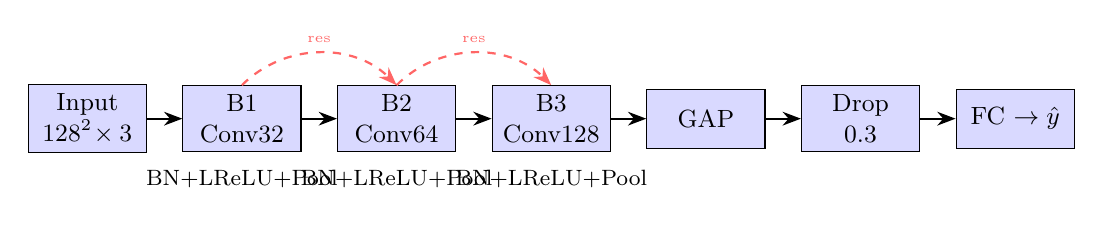
\begin{tikzpicture}[
  block/.style={rectangle, draw, fill=blue!15, minimum width=1.5cm, minimum height=0.75cm,
                font=\small, align=center},
  skip/.style={-Stealth, thick, dashed, bend left=45, color=red!60},
  arr/.style={-Stealth, thick}
]
\node[block] (inp) {Input\\$128^2\!\times3$};
\node[block, right=0.45cm of inp] (b1) {B1\\Conv32};
\node[block, right=0.45cm of b1]  (b2) {B2\\Conv64};
\node[block, right=0.45cm of b2]  (b3) {B3\\Conv128};
\node[block, right=0.45cm of b3]  (gap) {GAP};
\node[block, right=0.45cm of gap] (drop){Drop\\0.3};
\node[block, right=0.45cm of drop](fc)  {FC $\to\hat{y}$};
\draw[arr](inp)--(b1);\draw[arr](b1)--(b2);\draw[arr](b2)--(b3);
\draw[arr](b3)--(gap);\draw[arr](gap)--(drop);\draw[arr](drop)--(fc);
\draw[skip] (b1.north) to node[above,font=\tiny]{res} (b2.north);
\draw[skip] (b2.north) to node[above,font=\tiny]{res} (b3.north);
\node[below=0.1cm of b1,font=\footnotesize]{BN+LReLU+Pool};
\node[below=0.1cm of b2,font=\footnotesize]{BN+LReLU+Pool};
\node[below=0.1cm of b3,font=\footnotesize]{BN+LReLU+Pool};
\end{tikzpicture}
\caption{Model A architecture (298,369 parameters). LReLU = LeakyReLU($\alpha=0.01$).
Dashed red arrows are residual shortcuts. Dropout 0.3 applied after GAP.}
\label{fig:model_a}
\end{figure}

\subsubsection{Model B --- Best Four-Block Configuration}

Model B extends the architecture to four convolutional blocks with filter progression
$64 \to 128 \to 256 \to 512$, retaining the same regularisation choices (dropout 0.3,
residual connections, weight decay $10^{-4}$, LeakyReLU). Despite 16$\times$ more
parameters than Model A, Model B achieves a higher ablation MAE (4.07 vs 2.44), a finding
discussed in Section~\ref{sec:results_task1}. Total parameters: 4,861,953.

\begin{figure}[h]
\centering
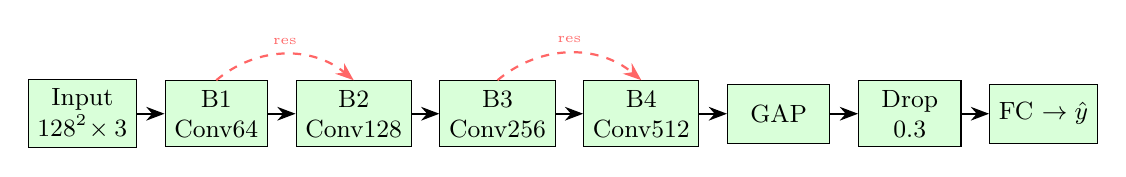
\begin{tikzpicture}[
  block/.style={rectangle, draw, fill=green!15, minimum width=1.3cm, minimum height=0.75cm,
                font=\small, align=center},
  skip/.style={-Stealth, thick, dashed, bend left=40, color=red!60},
  arr/.style={-Stealth, thick}
]
\node[block] (inp) {Input\\$128^2\!\times3$};
\node[block, right=0.35cm of inp] (b1) {B1\\Conv64};
\node[block, right=0.35cm of b1]  (b2) {B2\\Conv128};
\node[block, right=0.35cm of b2]  (b3) {B3\\Conv256};
\node[block, right=0.35cm of b3]  (b4) {B4\\Conv512};
\node[block, right=0.35cm of b4]  (gap) {GAP};
\node[block, right=0.35cm of gap] (drop){Drop\\0.3};
\node[block, right=0.35cm of drop](fc)  {FC $\to\hat{y}$};
\draw[arr](inp)--(b1);\draw[arr](b1)--(b2);\draw[arr](b2)--(b3);
\draw[arr](b3)--(b4);\draw[arr](b4)--(gap);\draw[arr](gap)--(drop);\draw[arr](drop)--(fc);
\draw[skip] (b1.north) to node[above,font=\tiny]{res} (b2.north);
\draw[skip] (b3.north) to node[above,font=\tiny]{res} (b4.north);
\end{tikzpicture}
\caption{Model B architecture (4,861,953 parameters). Same block structure as Model A
with one additional convolutional stage.}
\label{fig:model_b}
\end{figure}

\subsection{Ablation Study}
\label{sec:ablation}

A structured one-factor-at-a-time ablation was conducted over seven hyperparameter groups.
Each group fixes all other parameters at a common baseline and varies one factor.
SGD with momentum 0.9 and learning rate $10^{-3}$ is used throughout; each run trains
for up to 100 epochs with early stopping (patience = 10 on validation MAE).

\subsubsection{Group 0: Optimizer}

\begin{table}[h]
\centering
\caption{Effect of optimizer. Baseline: [32,64,128], $k=3$, no dropout, no residual.}
\begin{tabular}{lccc}
\toprule
Optimizer & Val MAE & Best Epoch & Params \\
\midrule
Adam & 21.32 & 60 & 93,825 \\
SGD  & \textbf{3.89} & 26 & 93,825 \\
\bottomrule
\end{tabular}
\end{table}

SGD outperforms Adam by a factor of 5.5. Adam's adaptive second-moment estimates appear
to converge prematurely on this small dataset. All subsequent groups use SGD.

\subsubsection{Group 1: Filter Progression and Depth}

\begin{table}[h]
\centering
\caption{Effect of filter progression and block count. Baseline: SGD, $k=3$, no dropout, no residual.}
\begin{tabular}{lccc}
\toprule
Filters & Blocks & Val MAE & Params \\
\midrule
{[}16, 32, 64{]}       & 3 & 2.97 &  23,873 \\
{[}32, 64, 128{]}      & 3 & \textbf{2.82} &  93,825 \\
{[}64, 128, 256{]}     & 3 & 3.96 & 371,969 \\
{[}16, 32, 64, 128{]}  & 4 & 4.99 &  98,049 \\
{[}32, 64, 128, 256{]} & 4 & 3.05 & 389,633 \\
\bottomrule
\end{tabular}
\end{table}

The [32, 64, 128] three-block network achieves the best MAE. Wider or deeper networks
without additional regularisation overfit. This configuration is used as the baseline
for all subsequent groups.

\subsubsection{Group 2: Residual Connections}

\begin{table}[h]
\centering
\caption{Effect of residual connections. Baseline: SGD, [32,64,128], $k=3$, no dropout.}
\begin{tabular}{lccc}
\toprule
Residual & Val MAE & Best Epoch & Params \\
\midrule
No  & 4.44 & 18 &  93,825 \\
Yes & \textbf{3.30} & 21 & 298,369 \\
\bottomrule
\end{tabular}
\end{table}

Residual connections reduce MAE by 26\% relative. The parameter increase arises from
$1\times1$ projection convolutions in the shortcuts. All subsequent groups include
residual connections.

\subsubsection{Group 3: Dropout Rate}

\begin{table}[h]
\centering
\caption{Effect of dropout rate. Baseline: SGD, [32,64,128], $k=3$, residual=True.}
\begin{tabular}{lcc}
\toprule
Dropout & Val MAE & Best Epoch \\
\midrule
0.0 & 5.03 & 12 \\
0.2 & \textbf{3.25} & 22 \\
0.3 & 4.67 & 20 \\
0.5 & 4.83 & 15 \\
\bottomrule
\end{tabular}
\end{table}

No dropout causes early stopping at epoch 12, consistent with overfitting on the training
set. Dropout 0.2 gives the lowest single-factor MAE. Subsequent groups use dropout 0.3
as a fixed baseline (the ablation design was not re-chained after each group); the final
selected config retains 0.3 because further improvements in Groups 5 and 6 were found
building on that baseline.

\subsubsection{Group 4: Kernel Size}

\begin{table}[h]
\centering
\caption{Effect of kernel size. Baseline: SGD, [32,64,128], dropout=0.3, residual=True.}
\begin{tabular}{lccc}
\toprule
Kernel & Val MAE & Best Epoch & Params \\
\midrule
$3\times3$ & 3.79 & 29 &    298,369 \\
$5\times5$ & 4.49 & 17 &    807,809 \\
$7\times7$ & \textbf{2.71} & 20 & 1,571,969 \\
\bottomrule
\end{tabular}
\end{table}

Kernel size 7 achieves the lowest MAE at 5.3$\times$ the parameter count of $k=3$.
Both selected models use $k=3$ to remain within the 1.5\,M parameter constraint and to
avoid fitting large-scale artefacts on a small training set.

\subsubsection{Group 5: Weight Decay}

\begin{table}[h]
\centering
\caption{Effect of L2 weight decay. Baseline: SGD, [32,64,128], $k=3$, dropout=0.3, residual=True.}
\begin{tabular}{lcc}
\toprule
$\lambda$ & Val MAE & Best Epoch \\
\midrule
$0$          & 3.75 & 29 \\
$10^{-5}$    & 3.03 & 24 \\
$10^{-4}$    & \textbf{2.81} & 12 \\
$10^{-3}$    & 3.32 & 21 \\
\bottomrule
\end{tabular}
\end{table}

Weight decay $\lambda = 10^{-4}$ reduces MAE by 25\% relative. Stronger decay
($10^{-3}$) over-regularises and degrades performance.

\subsubsection{Group 6: Activation Function}

\begin{table}[h]
\centering
\caption{Effect of activation. Baseline: SGD, [32,64,128], $k=3$, dropout=0.3, residual=True, $\lambda=10^{-4}$.}
\begin{tabular}{lcc}
\toprule
Activation & Val MAE & Best Epoch \\
\midrule
ReLU      & 3.21 & 20 \\
LeakyReLU & \textbf{2.44} & 44 \\
\bottomrule
\end{tabular}
\end{table}

LeakyReLU ($\alpha=0.01$) reduces MAE from 3.21 to 2.44. The later convergence epoch
(44 vs 20) is consistent with smoother gradient flow through the non-zero negative slope,
allowing the network to continue improving past the point where ReLU units become inactive.
This configuration represents the overall ablation winner and is adopted as \textbf{Model A}.

\subsection{Selected Model Configurations}

\begin{table}[h]
\centering
\caption{Final hyperparameter configurations. Model A is the best 3-block result from
ablation (Group 6 winner). Model B is the best 4-block result tested (ablation Group 8:
[64,128,256,512], same regularisation, MAE = 4.07 at epoch 11).}
\begin{tabular}{lll}
\toprule
Hyperparameter & Model A & Model B \\
\midrule
Filters        & {[}32, 64, 128{]}      & {[}64, 128, 256, 512{]} \\
Kernel size    & 3                      & 3 \\
Activation     & LeakyReLU              & LeakyReLU \\
Dropout        & 0.3                    & 0.3 \\
Residual       & Yes                    & Yes \\
Weight decay   & $10^{-4}$              & $10^{-4}$ \\
Optimizer      & SGD (momentum 0.9)     & SGD (momentum 0.9) \\
Learning rate  & $10^{-3}$              & $10^{-3}$ \\
Parameters     & 298,369                & 4,861,953 \\
Ablation MAE   & \textbf{2.44}          & 4.07 \\
\bottomrule
\end{tabular}
\label{tab:configs}
\end{table}

Model B achieves a higher MAE than Model A despite substantially more parameters.
This is consistent with the depth ablation (Group 1): adding convolutional blocks without
a proportional increase in training data increases overfitting. The available dataset
($\sim$750 training images) is insufficient to exploit 4.8\,M parameters effectively.

\subsection{Training Curves}
\label{sec:results_task1}

\begin{figure}[h]
\centering
\begin{subfigure}[b]{0.48\textwidth}
\fbox{\rule{0pt}{4cm}\rule{\textwidth}{0pt}}
\caption{Model A: train and val MAE over epochs.}
\end{subfigure}
\hfill
\begin{subfigure}[b]{0.48\textwidth}
\fbox{\rule{0pt}{4cm}\rule{\textwidth}{0pt}}
\caption{Model B: train and val MAE over epochs.}
\end{subfigure}
\caption{Training curves after full retraining on selected configurations.
\textbf{[Replace with training plots after final run]}.}
\label{fig:training_curves}
\end{figure}

\subsection{Quantitative Results}

\begin{table}[h]
\centering
\caption{Validation set performance after final training runs on selected configurations.}
\begin{tabular}{lcccc}
\toprule
Model & Val MAE & Val RMSE & Best Epoch & Params \\
\midrule
Model A & \textbf{[INSERT]} & \textbf{[INSERT]} & [INSERT] & 298,369 \\
Model B & \textbf{[INSERT]} & \textbf{[INSERT]} & [INSERT] & 4,861,953 \\
\bottomrule
\end{tabular}
\end{table}

\subsection{Qualitative Analysis}

\subsubsection{Success and Failure Cases}

\begin{figure}[h]
\centering
\fbox{\rule{0pt}{5cm}\rule{\linewidth}{0pt}}
\caption{GradCAM grid: each row shows the original image, GradCAM activation heatmap,
and overlay with predicted vs ground-truth count. Top rows: successes (low error);
bottom rows: failures (high error). \textbf{[Replace with gradcam.py output]}.}
\label{fig:gradcam}
\end{figure}

Failure cases are expected in two regimes: (1) very high seed density ($>100$ seeds per
image), where the spatial resolution after three pooling operations is insufficient to
resolve individual seeds; (2) images with illumination conditions not well represented in
the training distribution.

\subsubsection{GradCAM Visualisations}

GradCAM (Selvaraju et al., 2017) computes the gradient of the scalar output with respect
to the feature maps of the chosen convolutional layer, weighted by global-average-pooled
gradients:
\begin{equation}
  L_{\text{GradCAM}} = \text{ReLU}\!\left(\sum_k \alpha_k A^k\right),
  \quad
  \alpha_k = \frac{1}{Z}\sum_{i,j} \frac{\partial \hat{y}}{\partial A^k_{ij}}
\end{equation}
where $A^k$ is the $k$-th feature map and $Z$ its spatial size. Warm regions identify
the image areas most responsible for the predicted count.

\begin{figure}[h]
\centering
\fbox{\rule{0pt}{4cm}\rule{\linewidth}{0pt}}
\caption{GradCAM visualisations on six validation images using the last Conv block.
\textbf{[Replace with gradcam.py output]}.}
\end{figure}

\end{document}
